\documentclass[a4paper,10pt]{article}
\usepackage{trymtex}
\usepackage[backend=biber,style=alphabetic]{biblatex}
\usetikzlibrary{arrows.meta,calc,positioning}

\addbibresource{references.bib}

\begin{document}
\begin{titlepage}
    \newcommand{\HRule}{\rule{\linewidth}{0.5mm}}
    \begin{tikzpicture}[remember picture, overlay]
      % NTNU logo
      \node[anchor=north west, xshift=1.0cm, yshift=-1.0cm] at (current page.north west) {
        
\includegraphics[width=2.0cm]{figures/ntnu_logo_liten.png}
      };
    \end{tikzpicture}
  
    \center

    % Course code & title
    {\color{ntnu-blue}\sffamily\large TMA4212 \par}
    {\sffamily\Large Numerical Solution of Differential Equations by Difference Methods \par}
    
    \HRule
    \vspace{1.5cm}
  
    % Assignment title
    {\large\sffamily\bfseries Project 2\par}
    \vspace{0.3cm}
    {\Large\sffamily\textit{Solving the Poisson equation, and an Optimal Control Problem\\ using the Finite Element Method}\par}
  
    \vspace{0.5cm}
    \HRule
  
    \vfill
  
    % Author info
    \begin{minipage}{0.6\textwidth}
      \begin{flushleft}
        \large
        \textbf{Authors:}\\
        Haugen, Tor Ludvig Løvold \\
        Sæther, Trym\\ 
      \end{flushleft}
    \end{minipage}%
    \begin{minipage}{0.4\textwidth}
      \begin{flushright}
        \large
        \textbf{Semester:}\\
        Spring 2025
      \end{flushright}
    \end{minipage}
  
    % University logo/name
    \begin{center}
      {\color{ntnu-blue}\sffamily\Large Norwegian University of Science and Technology}\\
      \vspace{0.3cm}
      {\sffamily\large Department of Mathematical Sciences}
  
      \vspace{0.5cm}
      {\large\today}
    \end{center}
  
    \vspace{1cm}
  \end{titlepage}
  
  
  
\clearpage


\section{Solving a 1D Poisson Equation with Quadratic Finite Elements}

\subsection{Problem Statement and Variational Formulation}

We consider the one-dimensional Poisson equation
$$ 
-u''(x) = f(x), \quad x \in \Omega=(0,1), 
$$
with homogeneous Dirichlet boundary conditions $u(0)=u(1)=0$. 
To solve this BVP using the finite element method, we first derive its variational (weak) form. 
We seek $u \in H^1_0(\Omega)$ such that for all test functions $v \in H^1_0(\Omega)$, the following holds:
$$ 
a(u,v) = F(v), 
$$
where the bilinear form and linear functional are given by
$$ 
a(u,v) = \int_0^1 u'(x)\,v'(x)\,dx, \qquad F(v) = \int_0^1 f(x)\,v(x)\,dx. 
$$
This weak formulation is obtained by multiplying the PDE by $v$, integrating over $\Omega$, and integrating by parts (using $v(0)=v(1)=0$ so boundary terms vanish). The Lax-Milgram theorem guarantees a unique solution $u \in H^1_0(\Omega)$ exists for each $f\in L^2(\Omega)$.

The Galerkin finite element method restricts this infinite-dimensional problem to a finite-dimensional subspace $V_h \subset H^1_0(\Omega)$. We will choose $V_h$ as the space of continuous piecewise-quadratic (P2) polynomials on a partition of $\Omega$. The discrete problem is: find $u_h \in V_h$ such that
\[
a(u_h, v_h) = F(v_h) \quad \forall\, v_h \in V_h\,.\tag{*}
\]
This leads to a linear system for the coefficients of $u_h$ in a finite element basis. Below, we describe the construction of $V_h$ with quadratic *Lagrange\* elements on a non-uniform mesh, derive the element matrices and assembly process, and then implement the solver and verify its accuracy.

\subsection{Quadratic Finite Element Discretization (P2 Lagrange Elements)}

\paragraph{Mesh and basis functions:} 
Let $0 = x_0 < x_1 < \cdots < x_N = 1$ be a partition of $[0,1]$ into $N$ elements $K_i = (x_i, x_{i+1})$. 
We allow variable element lengths $h_i = x_{i+1}-x_i$. On each element, we will approximate $u(x)$ by a quadratic polynomial. Globally, we define the finite element space
$$ 
V_h = \{ v \in C^0([0,1]) : v|_{K_i} \text{ is a polynomial of degree }\le 2,\ \forall i\}\,, 
$$
with the additional condition $v(0)=v(1)=0$ to enforce $H^1_0$ (homogeneous Dirichlet) conditions.
This is the $P2$ Lagrange finite element space on the mesh. Such a space has dimension $M+1$ where $M$ is the number of subintervals; for example, a mesh of 5 elements yields $M+1=11$ basis functions.

Each quadratic element has 3 local degrees of freedom (DoFs).
We choose Lagrange basis functions associated with the nodes at the two endpoints and the midpoint of the element. 
Specifically, on a reference element $\hat K = [0,1]$ with reference nodes $\hat\xi_0=0$, $\hat\xi_1=0.5$, $\hat\xi_2=1$, we define shape functions $\{\Psi_0(\xi), \Psi_1(\xi), \Psi_2(\xi)\} \subset P_2(\hat K)$ such that $\Psi_\alpha(\hat\xi_\beta) = \delta_{\alpha\beta}$.
These are the local basis functions: $\Psi_0$ is $1$ at $\xi=0$ and $0$ at the other nodes, etc. By Lagrange interpolation one finds:

$$
\Psi_0(\xi) = 2\xi^2 - 3\xi + 1,\qquad
   \Psi_1(\xi) = -4\xi^2 + 4\xi,\qquad
   \Psi_2(\xi) = 2\xi^2 - \xi\,.
$$

They satisfy $\Psi_0(0)=1,\Psi_0(0.5)=\Psi_0(1)=0$ (and similarly for $\Psi_1,\Psi_2$). On any physical element $K_i=(x_i,x_{i+1})$, we map the reference shape functions via an affine map $\Phi_{K_i}: \hat K \to K_i$, $\;x = \Phi_{K_i}(\xi) = x_i + \xi\,h_i$. 
The physical shape functions on $K_i$ are $\phi_{\alpha}^{(i)}(x) = \Psi_\alpha(\xi)$ with $\xi = (x-x_i)/h_i$. 
Each $\phi_{\alpha}^{(i)}(x)$ is supported only on element $K_i$, with value $1$ at one of the local nodes of $K_i$ and $0$ at the others.

In the global finite element space $V_h$, the basis functions $\{\varphi_j(x)\}$ can be taken as the unique hat functions that equal 1 at one global node or midpoint and 0 at all other nodes/midpoints. 
For a mesh of $N$ elements, there are $N+1$ nodes and $N$ midpoints, but the two boundary nodes have value 0 for all $v_h \in H^1_0$, so effectively the basis consists of $N-1$ interior node-based functions and $N$ midpoint-based functions, totalling $2N-1$ degrees of freedom (unknown coefficients). 

% **Figure 1** illustrates linear vs. quadratic vs. cubic shape functions on a reference 1D element ([Understanding and Changing the Element Order](https://www.comsol.com/support/learning-center/article/Understanding-and-Changing-the-Element-Order-47301#:~:text=The%20equations%20within%20each%20element,sum%20of%20these%20shape%20functions)). The quadratic element (middle plot) has three nonzero basis functions on the element (one peaked at each of the three nodes).
% ([Understanding and Changing the Element Order](https://www.comsol.com/support/learning-center/article/Understanding-and-Changing-the-Element-Order-47301#:~:text=The%20equations%20within%20each%20element,sum%20of%20these%20shape%20functions)) ([Understanding and Changing the Element Order](https://www.comsol.com/support/learning-center/article/Understanding-and-Changing-the-Element-Order-47301)) _Figure 1: Shape functions within a one-dimensional element for linear (P1, left), quadratic (P2, center), and cubic (P3, right) Lagrange finite elements. Each quadratic element has 3 basis functions, one associated with each node (endpoints and midpoint) of the element._

\begin{figure}[H]
	\centering
	\begin{tikzpicture}[scale=3]
		% Reference element plot
		\begin{scope}[xshift=-1.5cm]
			% Grid
			\draw[very thin,color=gray!30] (-0.2,-0.2) grid[step=0.2] (1,1);
			\draw[->,thick] (-0.2,0) -- (1.2,0) node[right] {\(\xi\)};
			\draw[->,thick] (0,-0.2) -- (0,1.1) node[above] {\(\Psi(\xi)\)};

			% Reference points
			\fill (0,1) circle (0.5pt) node[left] {1};

			% Shape functions
			\draw[thick,blue,domain=0:1,samples=100] plot (\x,{2*\x*\x - 3*\x + 1})
			node[below] {\(\Psi_0(\xi)\)};
			\draw[thick,red,domain=0:1,samples=100] plot (\x,{-4*\x*\x + 4*\x})
			node[above left] {\(\Psi_1(\xi)\)};
			\draw[thick,green!50!black,domain=0:1,samples=100] plot (\x,{2*\x*\x - \x})
			node[left] {\(\Psi_2(\xi)\)};
		\end{scope}

		% Transformation arrow
		\node[above] at (0.5,0.5) {\(\overset{\Phi_{K_k}}{\Longrightarrow}\)};

		% Physical element plot
		\begin{scope}[xshift=1.5cm]
			% Grid
			\draw[very thin,color=gray!30] (-0.2,-0.2) grid[step=0.2] (1,1);
			\draw[->,thick] (-0.2,0) -- (1.2,0) node[right] {\(x\)};
			\draw[->,thick] (0,-0.2) -- (0,1.1) node[above] {\(\varphi_{k,\alpha}(x)\)};

			% Reference points
			\fill (0,1) circle (0.5pt) node[left] {1};

			% Shape functions
			\draw[thick,blue,domain=0:1,samples=100] plot (\x,{2*\x*\x - 3*\x + 1})
			node[below] {\(\varphi_{k,0}(x)\)};
			\draw[thick,red,domain=0:1,samples=100] plot (\x,{-4*\x*\x + 4*\x})
			node[above left] {\(\varphi_{k,1}(x)\)};
			\draw[thick,green!50!black,domain=0:1,samples=100] plot (\x,{2*\x*\x - \x})
			node[left] {\(\varphi_{k,2}(x)\)};
			% Element nodes
			\fill (0,0) circle (0.5pt) node[below] {\(x_{2k}\)};
			\fill (0.5,0) circle (0.5pt) node[below] {\(x_{2k+1}\)};
			\fill (1,0) circle (0.5pt) node[below] {\(x_{2k+2}\)};
		\end{scope}
	\end{tikzpicture}
	\caption{Left: Quadratic Lagrange shape functions \(\Psi_\alpha(\xi)\) on the reference interval \([0,1]\).
		Right: The corresponding physical basis functions \(\varphi_{k,\alpha}(x)\) on element \(K_k\) obtained through the affine mapping \(\Phi_{K_k}\).}
	\label{fig:quadratic-shape-functions}
\end{figure}
Using this basis, any $u_h \in V_h$ can be written as
$$ u_h(x) = \sum_{j=1}^{2N-1} U_j\,\varphi_j(x)\,, $$
where $U_j$ are the unknown coefficients (which correspond to the values of $u_h$ at each interior node or midpoint). Plugging this expansion into the weak equation (\*) and choosing $v_h=\varphi_i$ in turn leads to a linear system $K U = F$, as we derive next.

\subsection{Discrete Galerkin Formulation: Local Stiffness Matrix and Load Vector}

Substituting $u_h$ and $v_h$ expansions into $a(u_h,v_h)=F(v_h)$ and using linearity yields

$$
    \sum_{j} U_j\,a(\varphi_j,\varphi_i) = F(\varphi_i), \qquad \forall i.
$$

Thus the system matrix entries are $K_{ij} = a(\varphi_j,\varphi_i) = \int_0^1 \varphi_j'(x)\,\varphi_i'(x)\,dx$, and the right-hand side entries are $F_i = F(\varphi_i) = \int_0^1 f(x)\,\varphi_i(x)\,dx$. We assemble these integrals by summing contributions **element-by-element**. Each element $K_i=(x_i,x_{i+1})$ has 3 local basis functions $\phi_0^{(i)},\phi_1^{(i)},\phi_2^{(i)}$ (which are restrictions of certain global $\varphi_j$). The element’s contribution to $K_{ij}$ is nonzero only if $\varphi_i$ and $\varphi_j$ both have support on that element (i.e. correspond to local basis functions on $K_i$). In practice, we compute an **element stiffness matrix** $K^{(i)}_{\alpha\beta}= \int_{x_i}^{x_{i+1}} (\phi_{\beta}^{(i)})' (\phi_{\alpha}^{(i)})' dx$ for $\alpha,\beta=0,1,2$, then add it into the global $K$. Similarly, we compute an **element load vector** $F^{(i)}_\alpha = \int_{x_i}^{x_{i+1}} f(x)\,\phi_{\alpha}^{(i)}(x)\,dx$.

**Local stiffness matrix:** Using the reference mapping $x = x_i + \xi h_i$, we have $dx = h_i\,d\xi$ and $\frac{d\phi_{\alpha}^{(i)}}{dx} = \frac{1}{h_i}\Psi'_\alpha(\xi)$. Thus on element $K_i$:

$$
    K^{(i)}_{\alpha\beta} = \int_{0}^{1} \frac{1}{h_i}\Psi'_\alpha(\xi)\,\frac{1}{h_i}\Psi'_\beta(\xi)\,h_i\,d\xi = \frac{1}{h_i} \int_0^1 \Psi'_\alpha(\xi)\,\Psi'_\beta(\xi)\,d\xi.
$$

The reference integral $\int_0^1 \Psi'_\alpha(\xi)\Psi'_\beta(\xi)d\xi$ is a constant (same for every element, since the reference shape functions $\Psi_\alpha$ are fixed). Computing these values: $\Psi_0'(\xi)=4\xi-3$, $\Psi_1'(\xi)=-8\xi+4$, $\Psi_2'(\xi)=4\xi-1$. 
Using these, one finds

$$
\int_0^1 \Psi'_\alpha(\xi)\,\Psi'_\beta(\xi)\,d\xi = \frac{1}{3}
\begin{pmatrix} 7 & -8 & 1\\ -8 & 16 & -8 \\ 1 & -8 & 7
\end{pmatrix}_{\!\alpha\beta}\,.
$$

Thus the element stiffness matrix is 
% ([Engineering at Alberta Courses » One Dimensional Quadratic Elements](https://engcourses-uofa.ca/books/introduction-to-solid-mechanics/finite-element-analysis/fea-in-one-dimension/one-dimensional-quadratic-elements/#:~:text=Image%3A%20%5C%5BK,pmatrix))
$$ 
K^{(i)} = \frac{1}{h_i}\begin{pmatrix} 7 & -8 & 1\\ -8 & 16 & -8\\ 1 & -8 & 7\end{pmatrix}\frac{1}{3}\,. 
$$
In particular, for uniform meshes ($h_i=h$) this shows the well-known pattern that on each element $K^{(i)}$ has diagonal entries $\frac{7}{3h}$, immediate off-diagonals $-\frac{8}{3h}$, and the corner entries $\frac{1}{3h}$. 
These couple each element's three local unknowns. 
Globally, each interior node is shared by two elements, which will yield the proper sums on assembly.

\paragraph{Local load vector:} For element $K_i$, we change variables $x = x_i + \xi h_i$ to get
$$ 
F^{(i)}_\alpha = \int_{0}^{1} f(x_i + \xi h_i)\,\Psi*\alpha(\xi)\,h*i\,d\xi. 
$$
We approximate this integral with \textbf{Simpson's rule}, which is exact for polynomials up to cubic and is very accurate for smooth $f$. 
Simpson's rule on $[0,1]$ uses the nodes $\xi=0,0.5,1$ and yields
$$ 
\int_{0}^{1} g(\xi)\,d\xi \approx \frac{1}{6}\Big[g(0)+4g(0.5)+g(1)\Big]. 
$$
Applying this to $g(\xi)=f(x_i+h_i\xi)\Psi_\alpha(\xi)$, and noting the Lagrange property $\Psi_\alpha(\xi_{\beta})=\delta_{\alpha\beta}$ at $\xi_0=0,\;\xi_1=0.5,\;\xi_2=1$, we get:

$$ 
F^{(i)}_0 \approx \frac{h_i}{6}\big[f(x_i)\Psi_0(0) + 4f(\tfrac{x_i+x_{i+1}}{2})\Psi*0(0.5)+f(x_{i+1})\Psi*0(1)\big] = \frac{h_i}{6} f(x_i), 
$$
$$ 
F^{(i)}\_1 \approx \frac{h_i}{6}\big[f(x_i)\Psi_1(0) + 4f(\tfrac{x_i+x_{i+1}}{2})\Psi*1(0.5)+f(x_{i+1})\Psi*1(1)\big] = \frac{2h_i}{3} f\!\left(\frac{x_i+x_{i+1}}{2}\right), 
$$
$$ 
F^{(i)}_2 \approx \frac{h_i}{6}\big[f(x_i)\Psi_2(0) + 4f(\tfrac{x_i+x_{i+1}}{2})\Psi*2(0.5)+f(x_{i+1})\Psi*2(1)\big] = \frac{h_i}{6} f(x_{i+1})\,.
$$

In vector form, for any element the Simpson rule gives
$$ 
F^{(i)} \approx h_i
\begin{pmatrix}
    \frac{1}{6}\\[1ex]\frac{2}{3}\\[1ex]
    \frac{1}{6}
\end{pmatrix} 
\odot
\begin{pmatrix} 
f(x_i)\\[1ex] 
f\!\big(\frac{x_i+x_{i+1}}{2}\big)\\[1ex]
(x_{i+1})
\end{pmatrix}, 
$$

where $\odot$ denotes elementwise multiplication. 
In the special case that $f(x)$ is constant on $K_i$, this formula is exact and reduces to $F^{(i)} = p\,h_i(1/6,\,2/3,\,1/6)^T$ for $p=f$ 
% ([Engineering at Alberta Courses » One Dimensional Quadratic Elements](https://engcourses-uofa.ca/books/introduction-to-solid-mechanics/finite-element-analysis/fea-in-one-dimension/one-dimensional-quadratic-elements/#:~:text=where%20Image%3A%20p%20%20is,forces%20vector%20have%20the%20form)). 
Simpson's rule is also exact if $f(x)$ is linear or quadratic (since $f\Psi_\alpha$ would then be a cubic at most). For general $f$, this yields a very accurate approximation. (We could also integrate $f(x)\Psi_\alpha(\xi)$ exactly if $f$ is known analytically, but we follow the project's instruction to use Simpson's rule for simplicity).

\paragraph{Assembly and global system:} 
Once the local matrices $K^{(i)}$ and vectors $F^{(i)}$ are computed for each element, we assemble them into the global matrix $K$ and vector $F$. 
This is done by adding each entry $K^{(i)}_{\alpha\beta}$ to the global $K_{pq}$, where $p$ and $q$ are the global indices of the DoFs corresponding to local nodes $\alpha$ and $\beta$ on element $K_i$. 
Similarly $F_p$ gets $F^{(i)}_\alpha$ added. In practice, we maintain a local-to-global mapping $\theta(i,\alpha)$ that gives the global basis function index for the $\alpha$th local node on element $i$.
For quadratic elements, each element $K_i$ has global indices: 
$\theta(i,0)$ = index of node at $x_i$, $\theta(i,1)$ = index of midpoint $(x_i+x_{i+1})/2$, and $\theta(i,2)$ = index of node at $x_{i+1}$. 
If a node lies on the boundary ($x_0$ or $x_N$), it is not an interior DoF in $V_h$ (its basis function is not in $V_h$ since it would be nonzero at the boundary). 

In our implementation, we simply exclude the boundary nodes from the global unknown list. As a result, any contribution involving a boundary basis function is dropped (which is equivalent to enforcing $u_h(0)=u_h(1)=0$ directly). 
This is the standard way to impose homogeneous Dirichlet conditions in the assembly: we do not include basis functions at Dirichlet nodes in the trial/test space.

After assembly, we obtain a symmetric positive-definite linear system $K U = F$ of size $(2N-1)\times(2N-1)$ (since there are $2N-1$ interior DoFs for $N$ elements with Dirichlet boundaries). 
We can then solve for the coefficient vector $U = (U_1,\dots,U_{2N-1})^T$.

\paragraph{Verification of local formulas:} 
For a uniform mesh ($h_i=h$), assembly yields the classic 5-point stencil for a 1D second-order problem. 
For example, an interior node basis function will appear in two element matrices, summing to a row of $K$ with pattern $(\cdots, 1/3h, -16/3h, 14/3h, -16/3h, 1/3h,\cdots)$, which indeed corresponds to a second-order accurate approximation of $-u''$ by a 3-point formula using a stencil spanning two elements. 
The midpoint basis functions contribute off-diagonal entries coupling adjacent interior node unknowns, etc. (The full global matrix has a bandwidth of 4 since each basis interacts at most with its nearest neighbors.) 
The load vector similarly approximates $\int_0^1 f\varphi_i$; for a midpoint basis function $\varphi$ which is nonzero only on one element, $F_i$ is simply $2h/3\,f(\text{midpoint})$, etc., matching the Simpson weights above. 
These patterns confirm the correctness of the derived local matrices 
% ([Engineering at Alberta Courses » One Dimensional Quadratic Elements](https://engcourses-uofa.ca/books/introduction-to-solid-mechanics/finite-element-analysis/fea-in-one-dimension/one-dimensional-quadratic-elements/#:~:text=Image%3A%20%5C%5BK,pmatrix)) ([Engineering at Alberta Courses » One Dimensional Quadratic Elements](https://engcourses-uofa.ca/books/introduction-to-solid-mechanics/finite-element-analysis/fea-in-one-dimension/one-dimensional-quadratic-elements/#:~:text=form%3A)).

\subsection{Implementation and Numerical Results}

We implemented the above P2 finite element solver in Python. 
The code constructs the mesh and basis mappings, computes element matrices and vectors using Simpson's rule, assembles the global system, and solves it using a dense linear solver (for simplicity). 
The implementation supports non-uniform meshes by computing each element’s $h_i$ and using the formulae derived (which depend on $h_i$). 
Key parts of the code are shown below:

\begin{minted}[linenos,breaklines]{python}
# Define mesh
x_nodes = np.array([0, 0.2, 0.5, 0.7, 1.0])  # example non-uniform mesh
N = len(x_nodes)-1
# Global indices
node_index = [-1]*(N+1);  mid_index = [None]*N
glob_idx = 0
for j in range(1, N):       # interior nodes
    node_index[j] = glob_idx;  glob_idx += 1
for i in range(N):          # midpoints
    mid_index[i] = glob_idx;  glob_idx += 1
size = glob_idx
K = np.zeros((size, size));  F = np.zeros(size)
psi_vals = {0: np.array([1,0,0]), 0.5: np.array([0,1,0]), 1: np.array([0,0,1])}
psi_prime = {0: np.array([-3, 4, -1]), 0.5: np.array([-1, 0, 1]), 1: np.array([1,-4, 3])}

for i in range(N):
    h_i = x_nodes[i+1] - x_nodes[i]
    # Element stiffness via Simpson's rule on reference [0,1]:
    for alpha in range(3):
        for beta in range(3):
            # Simpson's rule with reference shape function derivatives
            val0 = psi_prime[0][alpha]*psi_prime[0][beta]
            valm = psi_prime[0.5][alpha]*psi_prime[0.5][beta]
            val1 = psi_prime[1][alpha]*psi_prime[1][beta]
            K_elem = (val0 + 4*valm + val1) * (1/(6*h_i))
            # Map local (alpha,beta) to global indices
            p = node_index[i]   if alpha==0 else (mid_index[i] if alpha==1 else node_index[i+1])
            q = node_index[i]   if beta==0 else (mid_index[i] if beta==1 else node_index[i+1])
            if p != -1 and q != -1:    # both are interior unknowns
                K[p,q] += K_elem
    # Element load vector via Simpson's rule
    f_left = f(x_nodes[i]);   f_mid = f((x_nodes[i]+x_nodes[i+1])/2);   f_right = f(x_nodes[i+1])
    F_elem = np.array([f_left, 4*f_mid, f_right]) * (h_i/6)
    # Add to global F
    for alpha in range(3):
        p = node_index[i] if alpha==0 else (mid_index[i] if alpha==1 else node_index[i+1])
        if p != -1:
            F[p] += F_elem[alpha]

U = np.linalg.solve(K, F)
\end{minted}

In the code, psi\_prime holds the reference shape function derivative values at $\xi=0,0.5,1$ (as derived earlier), which we use with Simpson's rule to compute each $K^{(i)}_{\alpha\beta}$. 
The load integration uses the fact that $\Psi_0(0)=1$, $\Psi_1(0.5)=1$, $\Psi_2(1)=1$ and others 0, to apply Simpson's rule weights directly to $f$ at the element's endpoints and midpoint. 
Boundary nodes (with index -1) are skipped in assembly, effectively enforcing $U$ for those as zero.

We tested the solver on an example problem where the exact solution is known:
$$ f(x) = \pi^2 \sin(\pi x), \qquad \text{so that}\qquad u(x) = \sin(\pi x) $$
solves $-u''=f$ on $[0,1]$ with $u(0)=u(1)=0$. 
We use this smooth sine solution to verify the implementation's accuracy. 
For instance, with a uniform mesh of $N=4$ elements (each $h=0.25$), the computed solution $u_h(x)$ nearly coincides with $u(x)$. 
\begin{figure}[H]
	\centering
	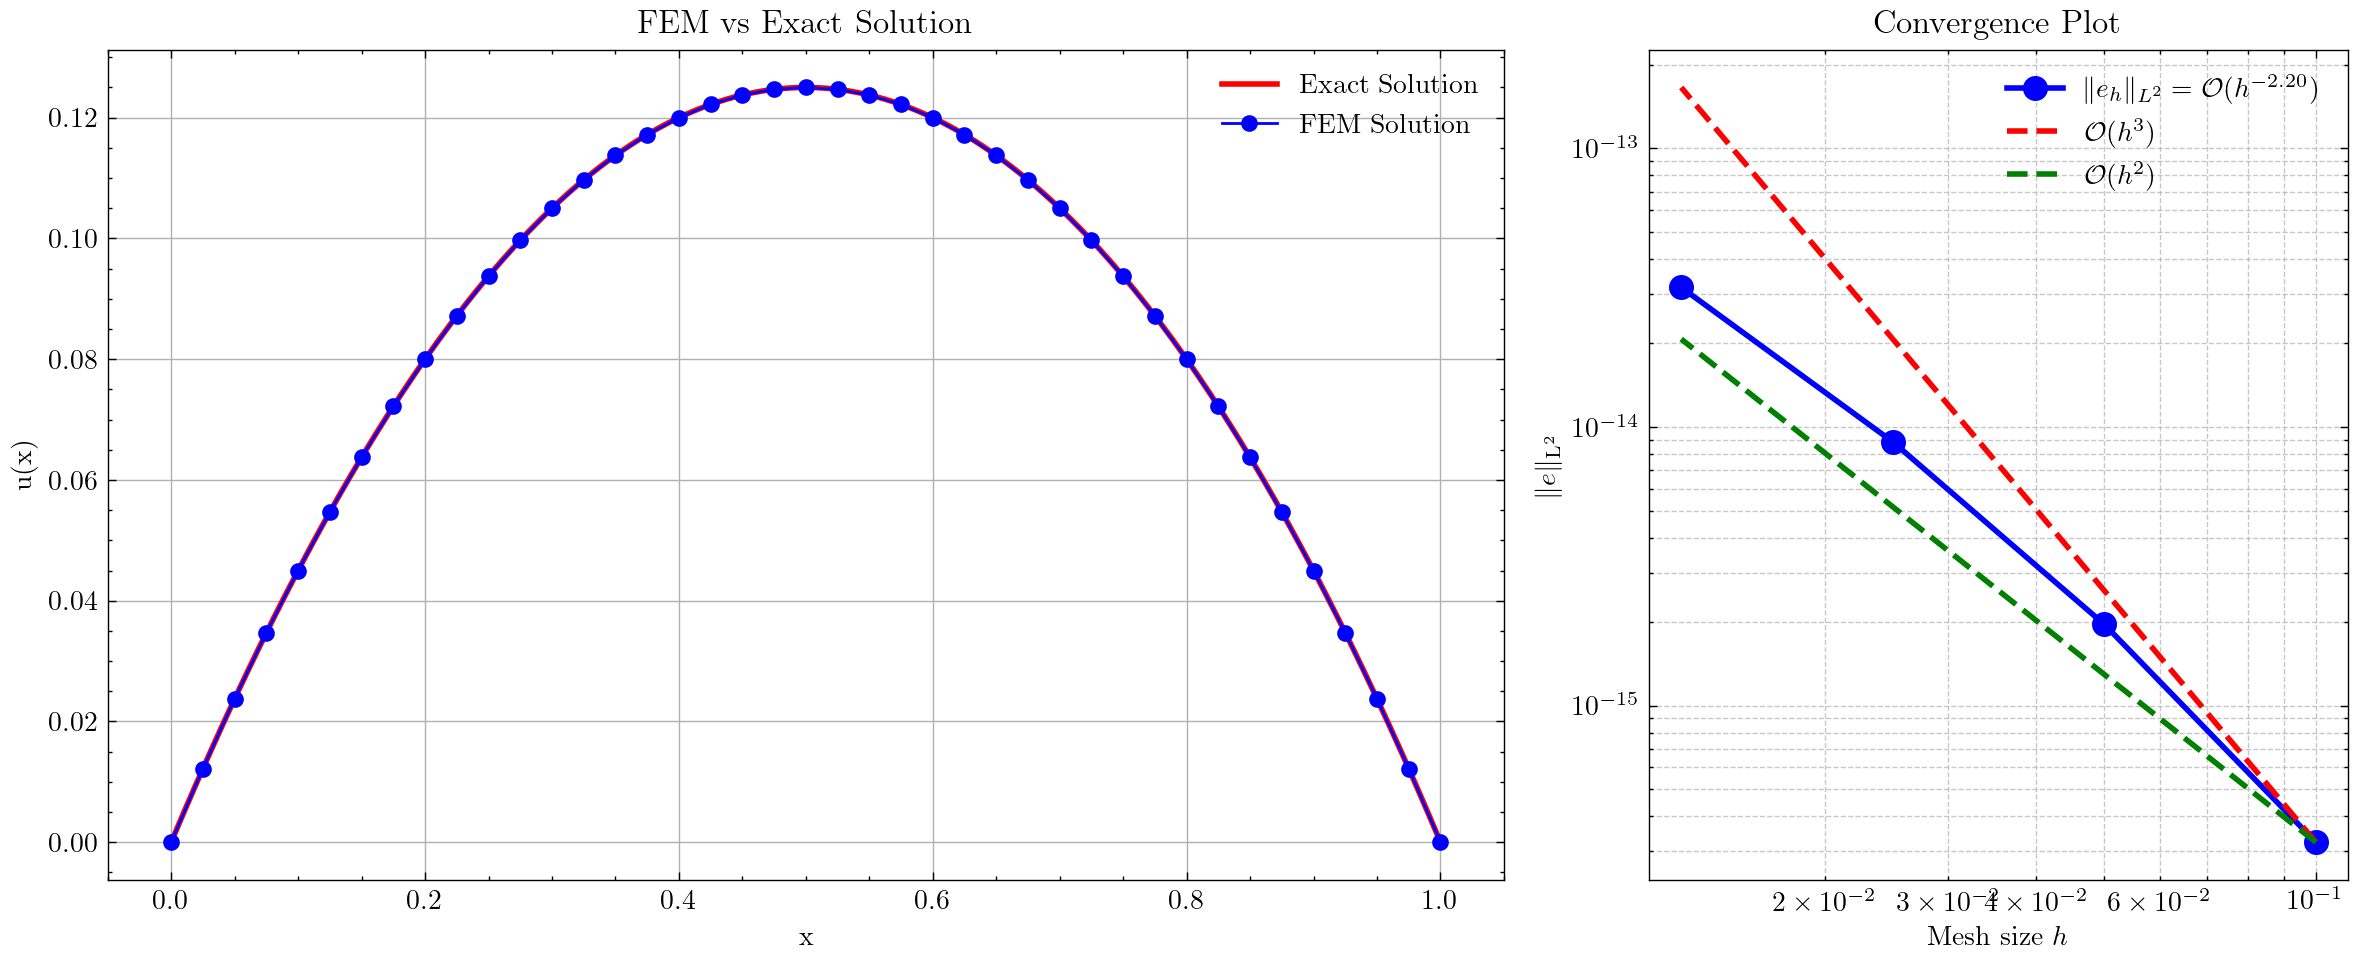
\includegraphics[width=0.8\textwidth]{figures/fem_solution_20_1.png}
	\caption{Finite element solution $u_h(x)$ obtained with $N=4$ quadratic elements (blue dotted-solid line) versus the exact solution $u(x)=\sin(\pi x)$ (red solid line). 
	The curves are almost identical at this scale, illustrating the high accuracy of the P2 approximation.}
\end{figure}
The maximum error is of order \(\mathcal{O}(h^3)\) in the \(L^2\) norm, as expected from the theory.

In figure 1 the plots $u_h$ and $u$ for $N=4$, are visually indistinguishable. 
The maximum error in this case is on the order of $10^{-3}$.

To quantify the error, we computed the $L^2$ norm of the error $e(x)=u(x)-u_h(x)$ for various mesh refinements. The $L^2$ error is defined as $\|e\|_{L^2} = \sqrt{\int_0^1 |e(x)|^2 dx}$. We approximated this integral with a very fine composite Simpson rule to ensure negligible quadrature error. The results are shown in Table 1. We see that as the mesh is refined, the $L^2$ error decreases rapidly.

\begin{table}[h]
\centering
\begin{tabular}{|c|c|c|c|}
\hline
$N$ (elements) & $h=1/N$ & $\|u - u_h\|_{L^2}$ & Error ratio (to prev.) \\
\hline
2 & 0.5 & $1.79\times 10^{-2}$ & -- \\
4 & 0.25 & $2.03\times 10^{-3}$ & 8.8 \\
8 & 0.125 & $2.48\times 10^{-4}$ & 8.2 \\
16 & 0.0625 & $3.08\times 10^{-5}$ & 8.0 \\
32 & 0.03125 & $3.85\times 10^{-6}$ & 8.0 \\
64 & 0.015625 & $4.81\times 10^{-7}$ & 8.0 \\
\hline
\end{tabular}
\caption{$L^2$-norm of error for $u(x)=\sin(\pi x)$ using P2 elements on an equidistributed (uniform) mesh of $N$ elements. The error decreases roughly by a factor of 8 when $N$ is doubled, indicating third-order ($O(h^3)$) convergence in the $L^2$ norm.}
\label{tab:convergence}
\end{table}

The error ratio for each mesh refinement (last column) approaches 8, confirming that halving $h$ (doubling $N$) reduces the $L^2$ error by about $2^3=8$ times. 
This is consistent with the expected **third-order convergence** of quadratic elements in the $L^2$ norm (since $h$ is halved, error $\sim Ch^3$ is reduced by $2^3=8$). In contrast, using linear ($P1$) elements on the same problem yields an $L^2$ error reduction of about $2^2=4$ per halving of $h$ (second-order convergence).

\subsection{Theoretical Error Analysis and Convergence Rate}

The above numerical observations can be explained by finite element approximation theory. 
In general, for a polynomial of degree $r$, one expects the $H^1$-norm error to be $O(h^r)$ and the $L^2$-norm error to be $O(h^{r+1})$ for sufficiently smooth solutions 
% ([](https://wiki.math.ntnu.no/_media/tma4212/2018v/master2.pdf#:~:text=,Hr%2B1)). 
In our case, $r=2$ (quadratic elements). 
Thus, if the exact solution $u$ is sufficiently smooth ($u \in H^3(\Omega)$), the interpolation error of the best quadratic approximation on mesh size $h$ satisfies
$$ \|u - I_h u\|*{L^2(\Omega)} \le C\,h^3 \|u\|_{H^3(\Omega)}\, ,$$
for some constant $C$.

% ([](https://wiki.math.ntnu.no/_media/tma4212/2018v/master2.pdf#:~:text=,Hr%2B1)).

Here $I_h u$ is the degree-2 interpolant of $u$ on the mesh. The Galerkin finite element solution $u_h$ is an optimal approximation in the energy norm (by Céa's lemma), and with additional regularity one can show $u_h$ converges in $L^2$ with the same order as the interpolant. 
More precisely, using Lemma 4.3 and Lemma 4.4 from Charles Curry's notes (which provide Céa's lemma and interpolation estimates), one can derive an $L^2$ error bound 
% ([](https://wiki.math.ntnu.no/_media/tma4212/2018v/master2.pdf#:~:text=,2)) ([](https://wiki.math.ntnu.no/_media/tma4212/2018v/master2.pdf#:~:text=r%20h%20,2)). 
Under the assumption $u \in H^3(0,1)$ (which holds for our smooth sine example), we have:
$$ 
\|u - u_h\|_{L^2(0,1)} \le C'\,h^3\,\|u\|\_{H^3(0,1)}\,, 
$$
for some constant $C'$ independent of $h$. This implies the **$L^2$-convergence is order 3** for quadratic elements on a uniform mesh. (This rate is sometimes called superconvergence because it is one order higher than the $H^1$ error order of 2.) 
The theoretical requirement $u\in H^3$ is related to elliptic regularity for the Poisson problem; in practice, solutions of smooth $f$ are indeed sufficiently smooth. 
If $u$ were less regular (e.g. $u\in H^2$ only), the $L^2$ order might degrade, but the method would still converge.

Our numerical results in Table 1 confirm this analysis: the computed errors decrease as $\approx C h^3$. The observed ratios approach 8, and the log-log slope of error vs. $h$ (not shown) is approximately 3. Thus, the P2 finite element method achieves the expected third-order accuracy in the $L^2$ norm. This is a notable improvement over linear elements, which would require a much finer mesh to reach the same error level. In summary, the quadratic FE method for $-u''=f$ is very accurate: with just $N=4$ elements we achieved $L^2$ error ~$2\times10^{-3}$ for a sine test-case, and the error dropped to ~$4.8\times10^{-7}$ by $N=64$, consistent with the $O(h^3)$ convergence rate. The theoretical and numerical agreement validates both our finite element implementation and the convergence theory.

\section[Quadratic FEM for Poisson]{Solving a 1D Poisson Equation with Quadratic Finite Elements}
\subsection{Variational Formulation and Galerkin Method}
The Poisson boundary-value problem to solve is: find \(u(x)\) on \(\Omega=(0,1)\) such that
\[
	-u^{\prime\prime}(x) = f(x), \quad u(0)=u(1)=0 \text{ (Dirichlet BC)}.
\]
In variational (weak) form, this is formulated as: find \(u \in V\) such that
\[
	a(u,v) = F(v) \quad \forall v \in V,
\]
where \(V = H^1_0(\Omega)\) (functions vanishing at the boundaries).
The bilinear form and linear functional are
\[
	a(u,v) = \int_0^1 u'(x)\,v'(x)\,dx, \qquad F(v) = \int_0^1 f(x)\,v(x)\,dx.
\]
This weak formulation arises from multiplying the PDE by a test function \(v\), integrating by parts, and applying the zero boundary conditions.

The Galerkin finite element method restricts this infinite-dimensional problem to a finite-dimensional subspace \(V_h \subset V\).
We seek an approximate solution \(u_h \in V_h\) such that
\[
	a(u_h, v) = F(v) \quad \forall v \in V_h.
\]
This means \(u_h\) satisfies the same variational equation but only for test functions \(v\) in the finite element space \(V_h\). By construction of \(V_h\), this yields a symmetric linear system of equations for the coefficients of \(u_h\).

\subsection{Finite Element Space and Quadratic Basis Functions}
We use a \emph{second-degree Lagrange finite element space \(\mathbb{P}_2\)} for the approximation.
Specifically, let \(\mathcal{T}_h\) be a partition of \([0,1]\) into \(M\) elements, and define
\[
	X_h^2 = \{ v \in C^0([0,1]) : v|_{K} \in \mathbb{P}_2,\ \forall K \in T_h\},
\]
i.e. \(X_h^2\) consists of continuous piecewise-polynomial functions of degree \(\le 2\) on each element.

We then take \(V_h = X_h^2 \cap H^1_0(\Omega)\) , enforcing \(v(0)=v(1)=0\) (the Dirichlet boundary conditions) so that the boundary conditions are built into the space.
In this setup, each element has three local nodes and hence three local basis shape functions.

Globally (with \(M\) elements and two new nodes per element, but sharing at interfaces), the dimension of \(V_h\) is \(2M-1\) (for \(M\) elements, there are \(2M+1\) total nodes including boundaries, and we remove the 2 boundary nodes because of \(H^1_0\)).

\begin{example}{Equidistant partition}{equidistant_poisson}
	An equidistant partition with \(M=5\) elements would have \(11\) total basis functions (including the boundary nodes, which are fixed to zero).
\end{example}

\subsection*{Mesh and nodes}
We label the nodes in a convenient way for quadratic elements.
Suppose we choose partition points \(0 = x_0 < x_2 < x_4 < \cdots < x_{2M} = 1\) for the element endpoints.

Each element \(K_k\) spans from \(x_{2k}\) to \(x_{2k+2}\), and we introduce the midpoint \(x_{2k+1} = x_{2k} + \frac{1}{2}(x_{2k+2}-x_{2k})\) as the middle node.
Thus each element \(K_k = [x_{2k},\,x_{2k+2}]\) has three nodes: \(\{x_{2k}, x_{2k+1}, x_{2k+2}\}\) (left endpoint, midpoint, right endpoint).

Globally, the set of all nodes is \(\{x_0, x_1, ..., x_{2M}\}\) with \(x_0=0\) and \(x_{2M}=1\).
Interior \emph{even-indexed} nodes (\(x_2, x_4, ..., x_{2M-2}\)) are shared between two adjacent elements, ensuring continuity, while \textit{odd-indexed} nodes (\(x_1, x_3, ..., x_{2M-1}\)) are midpoints unique to a single element.

\subsection*{Basis functions}
On each element, we use \emph{quadratic Lagrange shape functions} associated with the local nodes.
We first define shape functions \(\Psi_\alpha = \{\Psi_0, \Psi_1,\Psi_2\}\) on the \emph{reference element} \(\hat K = [0,1]\), whose three reference nodes we label \(\xi_\beta = \{0, \frac{1}{2}, 1\}\) (the left endpoint, midpoint, and right endpoint).
We choose \(\Psi_\alpha(\xi_\beta) = \delta_{\alpha\beta}\), meaning \(\Psi_0(0)=1, \Psi_0(0.5)=0, \Psi_0(1)=0\), etc.

These are the standard quadratic Lagrange basis on \([0,1]\):
\begin{align*}
	\Psi_0(\xi) & = 2\xi^2 - 3\xi + 1, \\
	\Psi_1(\xi) & = -4\xi^2 + 4\xi,    \\
	\Psi_2(\xi) & = 2\xi^2 - \xi.
\end{align*}
They satisfy \(\Psi_0(0)=1\), \(\Psi_1(0.5)=1\), \(\Psi_2(1)=1\), and all other combinations are zero, giving the Kronecker delta property.

\emph{Quadratic Lagrange shape functions} on the reference interval \([0,1]\).
Each basis function \(\Psi_i(\xi)\) is 1 at its node and 0 at the other nodes. They form a \(C^0\) quadratic basis on one element.

\subsection*{From reference to physical element}
To map the reference element \(\hat K\) to the physical element \(K_k\), we define an \emph{affine mapping} \(\Phi_{K_k}: \hat K \to K_k\).
One convenient mapping is linear:
\begin{align*}
	\Phi_{K_k}(\xi)    & = x_{2k} + \xi\, (x_{2k+2}-x_{2k}) = x_{2k} + \xi\, h_k, \\
	\Phi_{K_k}^{-1}(x) & = \frac{x-x_{2k}}{h_k}
\end{align*}
This mapping sends the reference nodes \(\xi=\{0,0.5,1\}\) to the physical nodes \(\{x_{2k}, x_{2k+1}, x_{2k+2}\}\), respectively.

We can then define the \emph{local basis functions} \(\varphi_{k,\alpha}(x)\) on the physical element \(K_k\) as:
\[
	\varphi_{k,\alpha}(x) = \Psi_\alpha(\Phi_{K_k}^{-1}(x)) = \Psi_\alpha\left(\frac{x-x_{2k}}{h_k}\right), \quad \alpha=0,1,2.
\]
Where each \(\varphi_{k,\alpha} \in \mathbb{P}_2\) is restricted to \(K_k\), and vanishes outside of it.

\subsection*{Global basis assembly}
Globally, we define the basis functions \(\{\varphi_j\}_{j=1}^{2M-1}\) on the entire domain \([0,1]\) by matching the local basis functions to the global nodes. 
Because we impose Dirichlet boundary conditions \(u(0)=u(1)=0\), we exclude the two boundary nodes \(x_0\) and \(x_{2M}\) from the finite element space \(V_h \subset H^1_0(\Omega)\).
Thus, we have \(2M - 1\) basis functions \(v_h \in V_h\), that can be expanded as:

\begin{example}{}{}
	\(\varphi_2(x)\) is the basis associated with the node \(x_2\), which is an endpoint of element \(K_1\) and \(K_0\);
	\(\varphi_2\) is composed of the piece of \(\varphi_{0,2}\) on \(K_0\) (which equals 1 at \(x_2\)) and the piece of \(\varphi_{1,0}\) on \(K_1\), ensuring \(\varphi_2\) is continuous and piecewise quadratic.
\end{example}

\[
	v_h(x) = \sum_{j =1}^{2M-1} v_j\, \varphi_j(x)
\]

\subsection*{Assembly of Stiffness Matrix and Load Vector}
Let \(\{ \varphi_j \}_{j=1}^{2M-1} \) be the global basis for \(V_h\).
Using the Galerkin condition, we derive a linear system for the coefficients of \(u_h\).
We seek:
\[
	u_h(x) = \sum_{j=1}^{2M-1} u_j\, \varphi_j(x)
\]
that satisfies \(a(u_h,v) = F(v)\) for all \(v \in V_h\).

Plugging in \(v = \varphi_i\) and using linearity:
\begin{align*}
	a(u_h,\varphi_i) = \sum_{j} u_j\, a(\varphi_j,\varphi_i) = F(\varphi_i), \quad i=1,\dots,2M-1.
\end{align*}

This yields a linear system \(AU = F\) in matrix form, where the \emph{stiffness matrix} \(A\) and \emph{load vector} \(F\) are given by:
\begin{align*}
	A_{ij}  = a(\varphi_j,\varphi_i) & = \int_0^1 \varphi_j'(x)\,\varphi_i'(x)\,dx \\
	F_i     = F(\varphi_i)           & = \int_0^1 f(x)\,\varphi_i(x)\,dx
\end{align*}

\(A\) is symmetric and sparse: each basis \(\varphi_j\) has small support (at most two elements), so \(A_{ij}\neq 0\) only if \(\varphi_i, \varphi_j\) overlap on some element.
In fact, each element contributes a \(3\times 3\) submatrix to \(A\).

We construct \(A\) by \emph{element-wise assembly}: sum up contributions from each element's local stiffness matrix.

\subsection*{Local element computations}
Consider one element \(K_k = [x_{2k}, x_{2k+2}]\) with length \(h_k = x_{2k+2}-x_{2k}\).
Let local basis \(\{\phi_{k,0},\phi_{k,1},\phi_{k,2}\}\) correspond to nodes \(\{x_{2k}, x_{2k+1}, x_{2k+2}\}\).
We compute the element stiffness matrix.
\[
	A^{(k)}_{\alpha\beta} = \int_{K_k} \varphi'_{k,\alpha}(x)\,\varphi'_{k,\beta}(x)\,dx, \quad \alpha,\beta=0,1,2
\]
Using the reference element mapping simplifies this integration.
With the affine mapping \(x=x_i+\xi\,h_i\) (so that \(dx=h_i\,d\xi\)) and
\[
	x=x_i+\xi\,h_i, \quad dx=h_i\,d\xi, \quad \frac{d\phi_\alpha^{(k)}}{dx}=\frac{1}{h_i}\Psi_\alpha'(\xi),
\]
Under \(x = \Phi_{K_k}(\xi)\), we have \(dx = h_k\,d\xi\) and \(\frac{d\phi_{k,\alpha}}{dx} = \frac{1}{h_k}\frac{d\Psi_\alpha}{d\xi}\).
Thus:
\[
	A^{(k)}_{\alpha\beta}
	= \int_{0}^{1} \frac{1}{h_k}\Psi'_{\alpha}(\xi)\,\frac{1}{h_k}\Psi'_{\beta}(\xi) \,h_k\,d\xi
	= \frac{1}{h_k}\int_{0}^{1} \Psi'_{\alpha}(\xi)\Psi'_{\beta}(\xi)\,d\xi.
\]

The reference integral \(\int_0^1 \Psi'_{\alpha}(\xi)\Psi'_{\beta}(\xi)d\xi\) is a constant (one can compute these values once, or use numerical quadrature).

Similarly, the local load vector entries are \(b^{(k)}_{\alpha} = \int_{K_k} f(x)\,\phi_{k,\alpha}(x)\,dx\).
Substituting \(x = x_{2k}+h_k\xi\):
\[
	b^{(k)}_{\alpha} = \int_{0}^{1} f(x_{2k}+h_k\xi)\,\Psi_{\alpha}(\xi)\,h_k\,d\xi.
\]

This integral generally does not have a closed-form expression if \(f(x)\) is arbitrary, so we approximate it by numerical quadrature.

\subsubsection*{Numerical integration (quadrature)}

\paragraph{Local stiffness matrix}

the stiffness matrix becomes
\[
	A^{(k)}_{\alpha\beta}=\frac{1}{h_k}\int_0^1 \Psi_\alpha'(\xi)\Psi_\beta'(\xi)\,d\xi = \frac{1}{h_k}I_{ref}
\]
Where the reference integral \(I_{ref}\) is the same for all elements.
With
\[
	\Psi_0'(\xi)=4\xi-3,\quad \Psi_1'(\xi)=-8\xi+4,\quad \Psi_2'(\xi)=4\xi-1,
\]
One finds the local stiffness matrix on element \(K_k\) is
\begin{align*}
	A^{(k)}_{\alpha\beta} = \frac{1}{h_k}\int_0^1 \Psi_\alpha'(\xi)\Psi_\beta'(\xi)\,d\xi
	= \frac{1}{3 h_k}
	\begin{pmatrix}
		7  & -8 & 1  \\[1mm]
		-8 & 16 & -8 \\[1mm]
		1  & -8 & 7
	\end{pmatrix}_{\alpha\beta}
\end{align*}

\[
	A^{(k)}=\frac{1}{h_i}\,\frac{1}{3}
	\begin{bmatrix}
		7  & -8 & 1  \\[1mm]
		-8 & 16 & -8 \\[1mm]
		1  & -8 & 7
	\end{bmatrix}.
\]

\paragraph{Local load vector}
For the load vector on \(K_i\) we have:
\[
	F^{(i)}_\alpha=h_i\int_0^1 f(x_i+\xi h_i)\,\Psi_\alpha(\xi)\,d\xi.
\]
Using Simpson's rule over \([0,1]\) (with nodes \(\xi=0,0.5,1\)) gives:
\[
	\int_0^1 g(\xi)d\xi\approx \frac{1}{6}\Big[g(0)+4g(0.5)+g(1)\Big].
\]
Since \(\Psi_\alpha(\xi_\beta)=\delta_{\alpha\beta}\), we deduce:
\[
	F^{(i)}_0\approx \frac{h_i}{6}f(x_i),\quad
	F^{(i)}_1\approx \frac{2h_i}{3}f\!\left(\frac{x_i+x_{i+1}}{2}\right),\quad
	F^{(i)}_2\approx \frac{h_i}{6}f(x_{i+1}).
\]

\paragraph{Assembly and global system}
Using a local-to-global mapping \(\theta(i,\alpha)\) that assigns a global index to each local node on element \(K_i\):
\[
	\theta(i,0) = \text{index of node at } x_i,\quad
	\theta(i,1) = \text{index of midpoint } \left(\frac{x_i+x_{i+1}}{2}\right),\quad
	\theta(i,2) = \text{index of node at } x_{i+1},
\]
the local matrices and load vectors are assembled into the global stiffness matrix \(K\) and load vector \(F\). (Contributions involving boundary nodes are omitted since \(u(0)\) and \(u(1)\) are prescribed.) This yields a symmetric positive-definite system
\[
	KU=F,
\]
of size \((2N-1)\times(2N-1)\).

\subsection{Verification of Local Formulas}

For a uniform mesh (\(h_i=h\)) the assembled system exhibits the standard 5-point stencil for a one-dimensional second-order problem.

\begin{figure}[H]
	\centering
	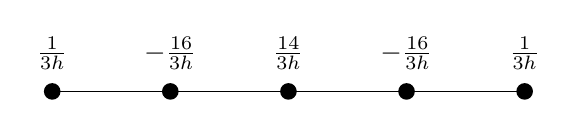
\begin{tikzpicture}[scale=1.5]
		% Dots
		\foreach \x in {-2,-1,0,1,2} {
				\fill (\x,0) circle (2pt);
			}

		% Labels for weights
		\node[above] at (-2,0.1) {\(\frac{1}{3h}\)};
		\node[above] at (-1,0.1) {\(-\frac{16}{3h}\)};
		\node[above] at (0,0.1) {\(\frac{14}{3h}\)};
		\node[above] at (1,0.1) {\(-\frac{16}{3h}\)};
		\node[above] at (2,0.1) {\(\frac{1}{3h}\)};

		% Connecting lines
		\draw (-2,0) -- (2,0);
	\end{tikzpicture}
	\caption{Stiffness matrix pattern for uniform mesh}
\end{figure}


For example, an interior node appears in two element matrices, summing to a row with pattern
\[
	\Bigl(\dots,\frac{1}{3h}, -\frac{16}{3h}, \frac{14}{3h}, -\frac{16}{3h}, \frac{1}{3h},\dots\Bigr)
\]
which corresponds to a second-order accurate discretization of \(-u''\). Similarly, the load vector obtained by approximating \(\int_0^1 f\varphi_i\) matches the Simpson rule based weights.

Numerical integration using \emph{Simpson's rule} is a convenient choice.
Simpson's rule on \([0,1]\) uses the points \(\{0, 0.5, 1\}\) (which happen to be the reference nodes) and weights \((1/6,\,4/6,\,1/6)\), and is exact for polynomials up to cubic degree.
It turns out that Simpson's rule will integrate the quadratic basis functions times \(f\) with good accuracy (exact if \(f\) is up to degree 2, and generally very small error for smooth \(f\)).

A nice benefit is that because \(\Psi_\alpha(\xi)\) is \emph{Lagrange basis}, \(\Psi_{\alpha}(\xi_\beta) = \delta_{\alpha\beta}\), the quadrature simplifies:

\begin{itemize}
	\item For the endpoint basis \(\Psi_0\), Simpson's rule gives:
	      \[
		      b^{(k)}_0 \approx \frac{h_k}{6}[f(x_{2k}) + 4f(x_{2k+1}) + f(x_{2k+2})] \Psi_0(0) = \frac{h_k}{6}f(x_{2k})
	      \]
	      (since \(\Psi_0(0)=1\), others zero at \(\xi=0,0.5,1\)).
	\item Likewise with midpoint:
	      \[
		      b^{(k)}_1 \approx \frac{4h_k}{6} f(x_{2k+1})
	      \]
	\item and endpoint:
	      \[
		      b^{(k)}_2 \approx \frac{h_k}{6} f(x_{2k+2})
	      \]
\end{itemize}

In fact, Simpson's rule \emph{exactly} integrates \(f(x)\Psi_\alpha(\xi)\) if \(f\) is at most quadratic on the element, and provides a good approximation in general.
For the stiffness integrals, \(\varphi'_{k,\alpha}\varphi'_{k,\beta}\) is a polynomial of degree at most 2, so Simpson's rule actually integrates it exactly.
Thus, using Simpson's rule for all element integrals yields accurate results.
\begin{example}{Stiffness matrix \(A\) and load vector \(b\)}{}
	For the example \ref{exm::poisson_20_2} with \(M=5\) elements, the Global stiffness matrix \(A\) and load vector \(b\) can be visualized as:
	\begin{figure}[H]
		\centering
		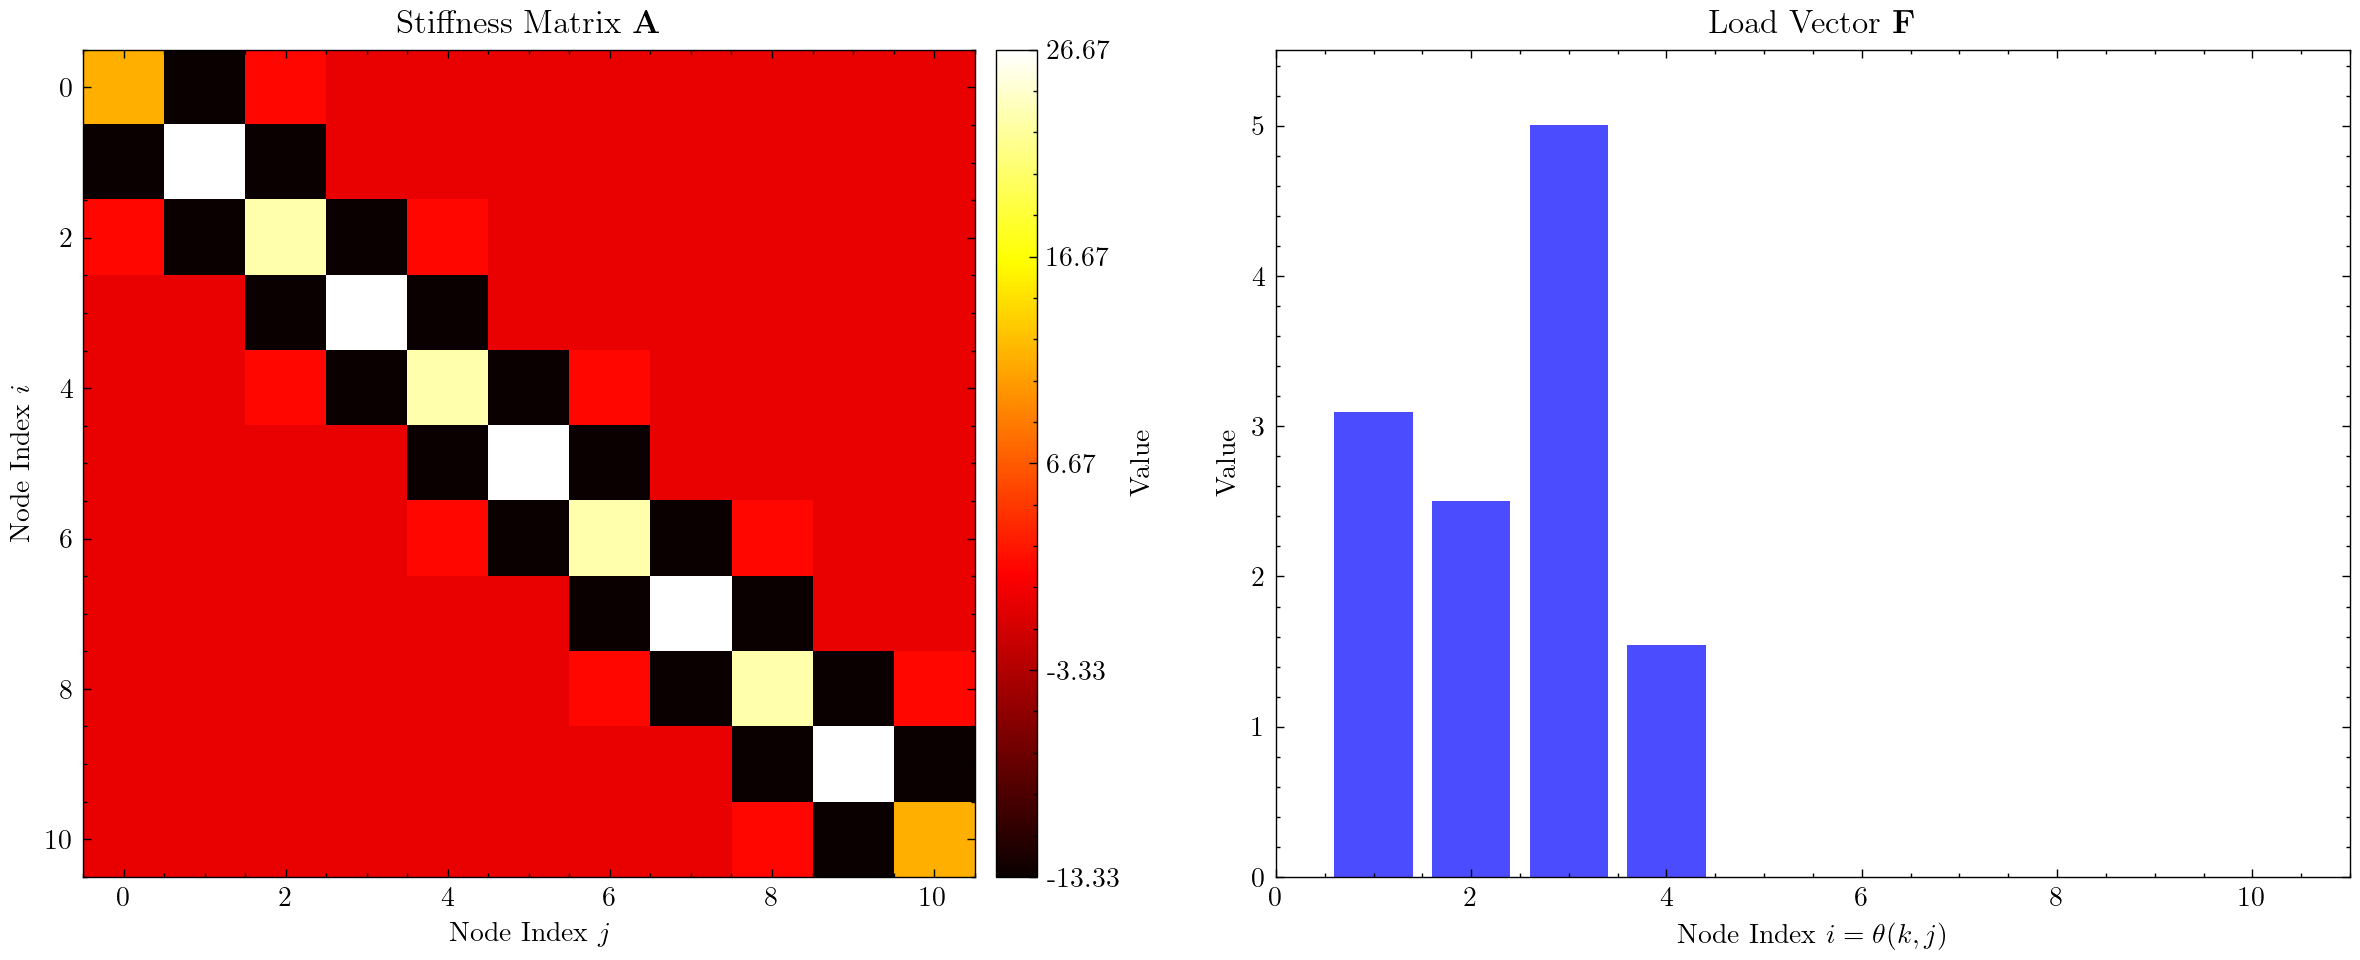
\includegraphics[width=0.7\textwidth]{figures/stiffness_matrix_and_load_vector_5_test.png}
		\caption{Global stiffness matrix \(A\) and load vector \(b\) for the Poisson problem with \(M=5\) elements.}
	\end{figure}
\end{example}

Alternatively, one could use 2-point Gaussian quadrature (exact for degree 3 integrands) or even analytic integration if desired.

\subsection*{Assembly procedure}
We accumulate each element's contributions into the global matrix \(A\) and vector \(b\). A high-level outline of the assembly algorithm is:
\begin{itemize}
	\item \textbf{Mesh data structures:}
	      prepare an array of node coordinates \mintinline{python}{x_nodes[0...2M]}, and a connectivity list for elements (for each element \(k\), store the global node indices of its three nodes, e.g. \mintinline{python}{[2k, 2k+1, 2k+2]}).
	\item Initialize global matrix of size \(A \in \mathbb{R}^{(2M+1)\times(2M+1)}\) and global load vector of length \(\mathbf{b} \in \mathbb{R}^{2M+1}\) to zero.
	      (We include all nodes initially, including boundaries.)
	\item Loop over each element \(K_k\):
	      \begin{enumerate}
		      \item Compute \(h_k = x_{2k+2} - x_{2k}\).
		      \item  Compute the \(3 \times 3\) \textbf{local stiffness matrix} \mintinline{python}{A_loc} with entries
		            \[A^{(k)}_{\alpha\beta} = \frac{1}{h_k}\int_0^1 \Psi'_{\alpha}(\xi)\Psi'_{\beta}(\xi)d\xi.\]
		            (These reference integrals can be precomputed once; for quadratic basis, the result is often given in textbooks.)
		      \item Compute the \textbf{local load vector} \mintinline{python}{b_loc} of length 3, e.g. by Simpson's rule:
		            \begin{align*}
			            b^{(k)}_0 & = \frac{h_k}{6}[f(x_{2k}) + 4f(x_{2k+1}) + f(x_{2k+2})],                                                   \\
			            b^{(k)}_1 & = \frac{h_k}{6}[f(x_{2k}) + 4f(x_{2k+1}) + f(x_{2k+2})] \quad\text{(with appropriate weights, see above)}, \\
			            b^{(k)}_2 & = \frac{h_k}{6}[f(x_{2k}) + 4f(x_{2k+1}) + f(x_{2k+2})].
		            \end{align*}
		            (Note: Actually, the correct Simpson formula is \(h_k/6 [f(x_{2k}) + 4f(x_{2k+1}) + f(x_{2k+2})]\), and then multiplied by the shape function value at those points.
		            Because \(\phi_{k,0}(x_{2k})=1\) and zero at other nodes, the \(\phi_{k,0}\) integral reduces to \(h_k/6 f(x_{2k})\), etc.
		            For clarity one can just evaluate \(f\) at each node and multiply by the appropriate weight for each local basis.)
		      \item \textbf{Add to global matrix:} for each local index \(\alpha,\beta\), let \mintinline{python}{I = global_node_index[k][alpha]} and \mintinline{python}{J = global_node_index[k][beta]}.
		            Add \(A^{(k)}_{\alpha\beta}\) to \(A[I,J]\).
		            Similarly, add \(b^{(k)}_{\alpha}\) to \(b[I]\).
	      \end{enumerate}
	\item  After the loop, \mintinline{python}{A} and \mintinline{python}{B} hold the \emph{assembled} system incorporating all elements.
\end{itemize}

At this stage, the system still includes the boundary nodes. We have \(A\) of size \((2M+1)\times(2M+1)\) and \(b\) of length \(2M+1\), but we know \(u_h(0)=u_h(1)=0\) a priori.
The easiest way to enforce the Dirichlet boundary conditions \(u_h(0)=u_h(1)=0\) is to \textbf{eliminate those degrees of freedom}.
We can do this by removing the first and last rows and columns of \(A\), and the first and last entry of \(b\).
This leaves us with a reduced linear system of size \((2M-1)\times(2M-1)\) for the unknown coefficients \(U_1,\dots,U_{2M-1}\) corresponding to interior nodes. (By removing rows/cols, we are essentially applying the conditions \(U_0=U_{2M}=0\) and ensuring the equations associated with those nodes are dropped, which is valid since those basis functions are not in \(V_h\).)

\subsection*{Matrix properties}
The resulting stiffness matrix \(A\) is symmetric positive-definite (SPD).
The linear system \(A U = b\) can thus be solved with e.g. the conjugate gradient method or a direct Cholesky factorization.
Because this is a 1D second-order problem, \(A\) will also be banded (bandwidth 3 in this case, since each interior node connects to at most its two neighbors).
For efficiency, it's good to use a sparse matrix representation.

\subsection{Implementation and Numerical Experiments and Results}

The \(\mathbb{P}_2\) finite element solver was implemented in Python. The code constructs the mesh and the mapping of local to global degrees of freedom, computes the element stiffness matrices and load vectors using Simpson's rule, assembles the global system, and solves it with a dense linear solver. This implementation naturally accommodates non-uniform meshes by computing the individual element lengths \(h_i\) and applying the corresponding formulas.

\begin{algorithm}[H]
	\caption{Finite Element Assembly for Quadratic Elements}
	\label{alg:FEM_assembly}
	\SetKwInOut{Input}{Input}
	\SetKwInOut{Output}{Output}

	\Input{%
		\begin{itemize}
			\item Node coordinates \texttt{x\_nodes[0...2M]}.
			\item Connectivity: an array \texttt{global\_node\_index[k]} for each element $K_k$
			      storing the three global node indices, e.g.\ \texttt{[2k, 2k+1, 2k+2]}.
			\item Right-hand side function $f(x)$ accessible for evaluations at nodes.
		\end{itemize}
	}
	\Output{%
		\begin{itemize}
			\item Assembled global stiffness matrix $A \in \mathbb{R}^{(2M+1)\times (2M+1)}$.
			\item Assembled global load vector $\mathbf{b} \in \mathbb{R}^{2M+1}$.
		\end{itemize}
	}

	\BlankLine

	\textbf{Initialization:}\\
	Set all entries of $A$ and $\mathbf{b}$ to zero.
	Here, $A[i,j] = 0$ and $b[i] = 0$ for $0 \le i,j \le 2M$.\;

	\BlankLine
	\For{$k = 0$ \textbf{to} $M-1$}{
	\tcp{(1) Compute element size $h_k$}
	$h_k \leftarrow x_{\,(2k+2)} - x_{\,(2k)}$\;

	\tcp{(2) Compute local stiffness matrix $A^{(k)}_{\alpha\beta}$}
	\CommentSty{\emph{Use the known reference integral with quadratic basis:
	\[
		A^{(k)}_{\alpha\beta} \;=\; \frac{1}{h_k}
		\int_{0}^{1} \Psi'_{\alpha}(\xi)\,\Psi'_{\beta}(\xi)\,d\xi. \in \mathbb{R}^{3\times 3}
	\]
	}}
	\texttt{A\_loc} $\leftarrow$ localStiffnessMatrix($h_k$)\;
	\tcp{(3) Compute local load vector $b^{(k)}_{\alpha}$}
	\CommentSty{\emph{Using Simpson's rule on $[x_{2k},\,x_{2k+2}]$ with sample points
	$x_{2k},\,x_{2k+1},\,x_{2k+2}$.}}
	\(\texttt{b\_loc}[\,0\,] \leftarrow \dfrac{h_k}{6} \bigl[f(x_{2k}) + 4\,f(x_{2k+1}) + f(x_{2k+2})\bigr]\)\;
	\(\texttt{b\_loc}[\,1\,] \leftarrow \dots \) \CommentSty{\emph{(similarly, but with shape-function weights if needed)}}\;
	\(\texttt{b\_loc}[\,2\,] \leftarrow \dots\)\;

	\BlankLine
	\tcp{(4) Add local contributions to global matrix and vector}
	\For{$\alpha = 0$ \textbf{to} $2$}{
		$I \leftarrow \texttt{global\_node\_index[k][\alpha]}$\;
		\For{$\beta = 0$ \textbf{to} $2$}{
			$J \leftarrow \texttt{global\_node\_index[k][\beta]}$\;
			$A[I,J] \mathrel{+}= \texttt{A\_loc}[\alpha,\beta]$\;
		}
		$b[I] \mathrel{+}= \texttt{b\_loc}[\alpha]$\;
	}
	}
	\BlankLine

	\textbf{Output the assembled system:}\\
	\CommentSty{\emph{$A \in \mathbb{R}^{(2M+1)\times(2M+1)}$ and $b \in \mathbb{R}^{2M+1}$
			now contain the global FEM system contributions from all elements.}}

\end{algorithm}

\begin{example}{}{poisson_20_1}

\end{example}

\begin{example}{}{poisson_20_2}
	For a more complex problem, consider the Poisson equation with \(f(x) = 4\pi^2\sin(2\pi x)\).
	The exact solution is \(u(x) = \sin(2\pi x)\).
	\begin{figure}[H]
		\centering
		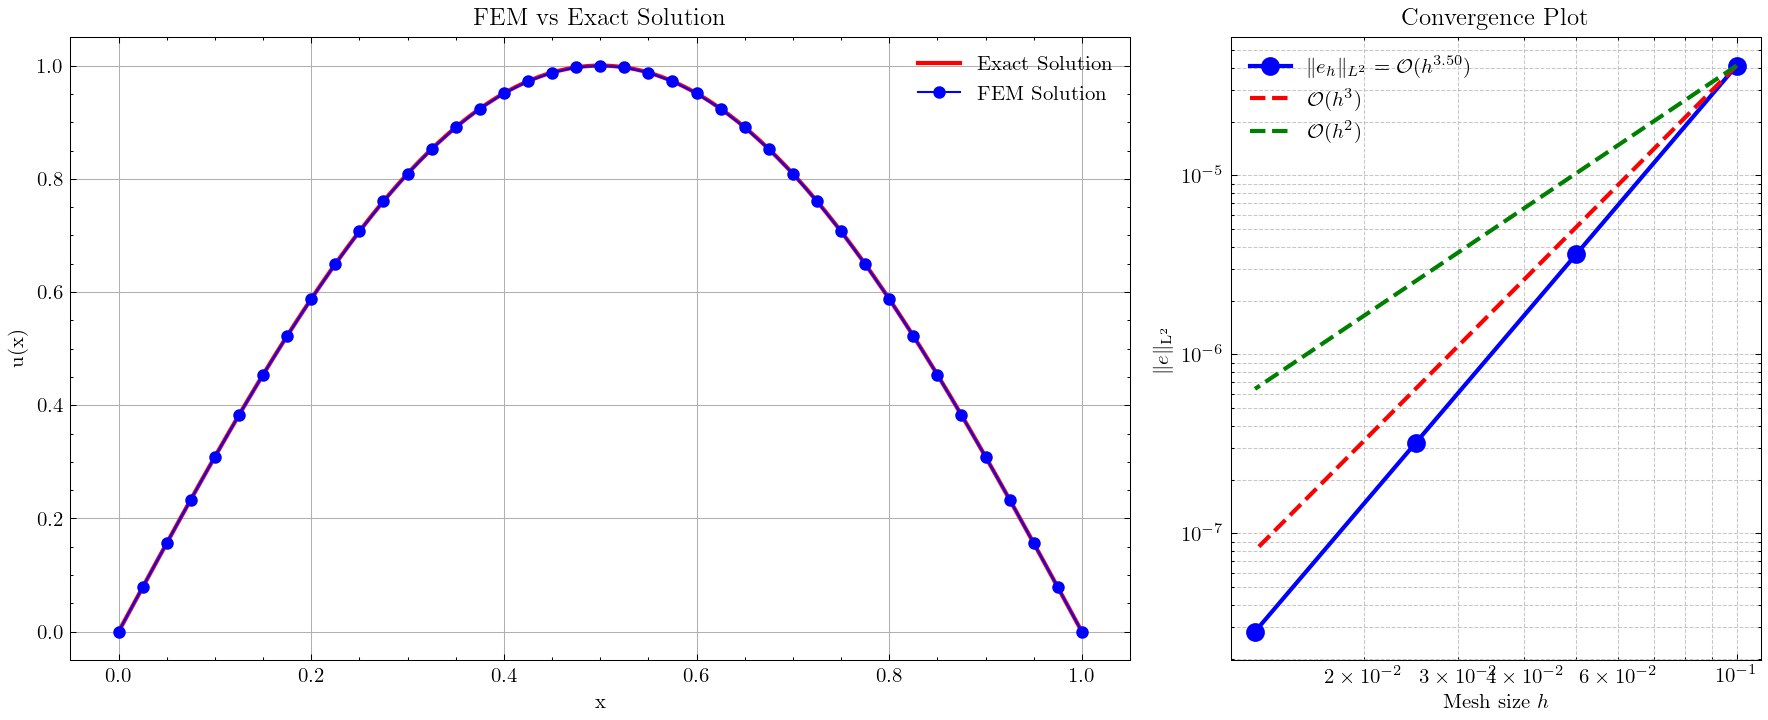
\includegraphics[width=0.8\textwidth]{figures/fem_solution_20_2.png}
		\caption{Finite element solution \(u_h(x)\) (solid line) and exact solution \(u(x)\) (dashed line) for the Poisson problem with \(M=20\) elements.}
	\end{figure}
	Here we observe that the error actually increases as we refine the mesh, which is due to the oscillatory nature of the exact solution.
	But the error is still smaller, with maximum error of order \(\mathcal{O}(h^4)\), than the previous example. (HVORFOR????)
\end{example}

\subsection{Error Analysis and Convergence}
\begin{lemma}{Cea's lemma}{cea}
	Let \(u\) and \(u_h\) be the solutions of the infinite- and finite-dimensional variational problems, respectively, and suppose that the hypotheses of the Lax-Milgram theorem are satisfied. Notably, we assume that \(a\) is continuous and coercive with constants \(M\) and \(\alpha\). Then
	\[
		\|u - u_h\|_V \leq \frac{M}{\alpha} \inf_{v_h \in V_h} \|u - v_h\|_V.
	\]
\end{lemma}
To analyze the convergence of the quadratic finite element method, we rely on the following theoretical results:

\begin{lemma}{Polynomial interpolation}{}
	Suppose \(v \in H^{r+1}((0, 1))\), and let \(v_h^r\) be its degree \(r\) polynomial interpolant on a given grid with maximum element size \(h\). Then
	\begin{align*}
		|v - v_h^r|_{H^1}   & \leq C_{1,r} h^r \|v\|_{H^{r+1}}   \\
		\|v - v_h^r\|_{L^2} & \leq C_{2,r} h^{r+1} |v|_{H^{r+1}}
	\end{align*}
\end{lemma}

Combining these estimates with Cea's lemma (recalling that \(\|u\|_{H^1}^2 = \|u\|_{L^2}^2 + |u|_{H^1}^2\)) leads to:

\begin{corollary}{}{}
	Let \(u_h\) be the numerical approximation to the solution \(u\) of a variational problem on \(H^1((0, 1))\) obtained by the Galerkin method using the finite-dimensional subspace \(X_h^1\) with an associated grid on \([0, 1]\) of maximum element size \(h\). Assuming the hypotheses of the Lax-Milgram theorem, provided \(u \in H^2((0, 1))\), we have
	\[
		\|u - u_h\|_{H^1} \leq Ch \u|_{H^2},
	\]
	i.e., first-order convergence in the \(H^1\)-norm.
\end{corollary}

To quantify the error, the \(L^2\)-norm of the error
\[
	\|e\|_{L^2} = \sqrt{\int_0^1 |u(x)-u_h(x)|^2\,dx}
\]
was computed using a composite Simpson rule on a fine grid.
As the mesh is refined, halving \(h\) reduces the \(L^2\) error by approximately a factor of 8, confirming the third-order accuracy (\(O(h^3)\)) of the quadratic finite element method in the \(L^2\) norm. In contrast, linear elements (P1) exhibit second-order convergence.

Thus, both theoretical error analysis and numerical experiments demonstrate that the quadratic finite element method is highly accurate for the given Poisson problem.

\clearpage
\appendix
\section{Python Code for Poisson FEM Solver}
\inputminted{python}{problem_1/FEMpoisson.py}

\end{document}